SymPy includes several packages that allow users to solve domain specific
problems. For example, a comprehensive physics package is included that is
useful for solving problems in classical mechanics, optics, and quantum
mechanics along with support for manipuating physical quantities with units.


\subsection{Classical Mechanics}

\subsubsection{Vector Algebra}

The \verb|sympy.physics.vector| package provides reference frame, time, and
space aware vector and dyadic objects that allow for three dimensional
operations such as addition, subtraction, scalar multiplication, inner and
outer products, cross products, etc. Both of these objects can be written in
very compact notation that make it easy to express the vectors and dyadics in
terms of multiple reference frames with arbitrarily defined relative
orientations. The vectors are used to specify the positions, velocities, and
accelerations of points, orientations, angular velocities, and angular
accelerations of reference frames, and force and torques. The dyadics are
essentially reference frame aware $3 \times 3$ tensors. The vector and dyadic
objects can be used for any one-, two-, or three-dimensional vector algebra and
they provide a strong framework for building physics and engineering tools.

The following Python interpreter session showing how a vector is created using
the orthogonal unit vectors of three reference frames that are oriented with
respect to each other and the result of expressing the vector in the $A$
frame. The $B$ frame is oriented with respect to the $A$ frame using Z-X-Z
Euler Angles of magnitude $\pi$, $\frac{\pi}{2}$, and
$\frac{\pi}{3}$\si{\radian}, respectively whereas the $C$ frame is oriented
with respect to the $B$ frame through a simple rotation about the $B$ frame's
X unit vector through $\frac{\pi}{2}$\si{\radian}.

\begin{verbatim}
>>> from sympy import pi
>>> from sympy.physics.vector import ReferenceFrame
>>> A = ReferenceFrame('A')
>>> B = ReferenceFrame('B')
>>> C = ReferenceFrame('C')
>>> B.orient(A, 'body', (pi, pi / 3, pi / 4), 'zxz')
>>> C.orient(B, 'axis', (pi / 2, B.x))
>>> v = 1 * A.x + 2 * B.z + 3 * C.y
>>> v
A.x + 2*B.z + 3*C.y
>>> v.express(A)
A.x + 5*sqrt(3)/2*A.y + 5/2*A.z
\end{verbatim}

\subsubsection{Mechanics}

The \verb|sympy.physics.mechanics| package utilizes the \texttt{sympy.\allowbreak{}physics.\allowbreak{}vector} package
to populate time aware particle and rigid body objects to fully describe the
kinematics and kinetics of a rigid multi-body system. These objects store all
of the information needed to derive the ordinary differential or differential
algebraic equations that govern the motion of the system, i.e., the equations
of motion. These equations of motion abide by Newton's laws of motion and can
handle any arbitrary kinematical constraints or complex loads. The package
offers two automated methods for formulating the equations of motion based on
Lagrangian Dynamics~\cite{Lagrange1811} and Kane's Method~\cite{Kane1985}. Lastly, there
are automated linearization routines for constrained dynamical
systems based on~\cite{Peterson2014}.

\subsection{Symbolic Quantum Mechanics}

The \verb|sympy.physics.quantum| package provides python objects for defining and manipulating quantum functions, states, operators, including options to manipulate quantum states. One can, for example, define general operators and apply commutation relations to them.
\begin{verbatim}
>>> from sympy.physics.quantum import Commutator, Dagger, Operator
>>> A = Operator('A')
>>> B = Operator('B')
>>> comm = Commutator(A, B)
>>> comm
[A,B]
>>> comm.doit()
A*B - B*A
\end{verbatim}
The commutator orders its objects in canonical order, factoring out commutative constants. The commutator objects can expand commutator expressions, and can properly apply adjoint operators.
\begin{verbatim}
>>> Dagger(Commutator(C+B, A)).expand(commutator=True)
[Dagger(A),Dagger(B)] + [Dagger(A),Dagger(C)]
\end{verbatim}

The \verb|sympy.physics.quantum| package provides features to create and manipulate qubit states for quantum information theory.
\begin{verbatim}
>>> from sympy.physics.quantum.qubit import Qubit
>>> Qubit(0,0,0)
|000>
>>> q = Qubit('0101')
>>> q
|0101>
\end{verbatim}
Qubit states can be manipulated in standard ways, flipping spins, applying adjoint operations, and forming tensor and inner products.
\begin{verbatim}
>>> from sympy.physics.quantum.dagger import Dagger
>>> q.flip(1)
|0111>
>>> Dagger(q)
<0101|
>>> ip = Dagger(q)*q
>>> ip
<0101|0101>
>>> ip.doit()
1
\end{verbatim}
Quantum operators can be applied to transform these states.
\begin{verbatim}
>>> from sympy.physics.quantum.qubit import Qubit, measure_all
>>> from sympy.physics.quantum.gate import H, X, Y, Z
>>> from sympy.physics.quantum.qapply import qapply
>>> c = H(0)*H(1)*Qubit('00')
>>> c
H(0)*H(1)*|00>
>>> q = qapply(c)
>>> measure_all(q)
[(|00>, 1/4), (|01>, 1/4), (|10>, 1/4), (|11>, 1/4)]
\end{verbatim}

\begin{figure}[htbp]
\begin{center}
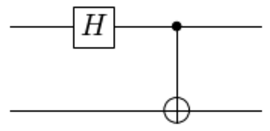
\includegraphics[scale=0.75]{images/circuitplot-example}
\caption{Example of plotting a simple quantum circuit.}
\label{fig-circuitplot-example}
\end{center}
\end{figure}

Finally, there are also capabilities to plot circuit diagrams for simple circuits.
\begin{verbatim}
>>> from sympy.physics.quantum.circuitplot import CircuitPlot
>>> from sympy.physics.quantum.gate import H, CNOT
>>> CircuitPlot(CNOT(1,0)*H(1),2)
\end{verbatim}
This results in Figure~\ref{fig-circuitplot-example}.
